\section{Tâches effectuées}

Durant mon stage, j'ai réalisé différentes tâches touchant à différents
domaines. Ces tâches, j'ai eu la liberté de les choisir (en fonction des besoins
de Be Sport et de la répartition de celles-ci) au fur et à mesure des quatres
mois passés chez Be Sport. Certaines tâches, que je qualifierai de mineures et
majoritairement dans Ocsigen Start, étaient ajoutées aux tâches principales.

Pendant tout mon stage, je n'ai jamais contribué directement au code de la
plateforme Be Sport: le travail que j'effectuais était principalement dans Ocsigen Start
(que Be Sport utilise comme base) ou dans un projet séparé (comme pour les push
notifications) et celui-ci était utilisé par un développeur de Be Sport comme
base. Cette méthode a été choisie par Vincent Balat pour que je puisse être
productif plus rapidement car sinon, j'aurais du, en plus du projet Ocsigen qui
est déjà assez conséquent, comprendre l'ensemble de Be Sport.

\subsection{OAuth2.0 et OpenID Connect}

Lorsque je suis arrivé le premier jour, j'ai pu choisir une première tâche dans
une liste de prochaines fonctionnalités devant être développées dans Be Sport.

J'ai choisi l'implémentation d'un système semblable à Facebook
Login\cite{facebook-login} dans Be Sport, appelée Be Sport Connect\footnote{La dénomination n'a pas été officiellement
  choisie mais celle-ci était utilisée pour parler de cette fonctionnalité.}.
Cette fonctionnalité doit permettre à des applications indépendantes de Be Sport
de pouvoir utiliser un compte créé sur Be Sport sans que l'utilisateur donne, à
nouveau, certaines informations comme son adresse email, son nom, son prénom et
un mot de passe et sans pour autant accéder à
toutes les données possédées par Be Sport sur l'utilisateur (comme certains
sites font avec Facebook, LinkedIn, Twitter ou encore GitHub).\footnote{Par la
suite (après 6 semaines de stage), les
  priorités de Be Sport ont changé
  et j'ai donc laissé de côté cette partie pour me focaliser sur Ocsigen Start
  et les push notifications, tâches décrites ci-dessous. Vers la fin de mon
  stage, le travail a été repris pour mettre à jour avec les changements
  d'Ocsigen Start. Cependant, l'implémentation, bien que très avancée, n'est pas
encore finie.}.
L'idée derrière cette fonctionnalité est de séparer l'application Be Sport en
plusieurs applications indépendantes. Par exemple, le tchat Be Sport, actuellement
dépendant de Be Sport, pourrait être une application entièrement séparée de Be
Sport sous le nom de \emph{Be Sport Chat}. Un autre exemple est une application
\emph{Be Sport Location} qui permet de localiser un utilisateur connecté et
lister les différents événements proches de lui. Ces deux applications ont
besoin de créer des comptes pour retenir diverses informations, d'où l'intérêt
de Be Sport Connect pour éviter de devoir créer des comptes séparés pour les
deux applications en plus de Be Sport.


\subsection{JWT : Json Web Token}

Comme dit précédemment, OpenID Connect utilise le standard JWT (Json Web
Token)\cite{official-jwt-website, official-openid-connect-website, rfc-jwt}
pour représenter de manière sécurisée des demandes (\textbf{claims} en anglais) et les
transférer entre deux applications en utilisant des \textit{jetons} (ou
\textit{token} en anglais).
Aucune bibliothèque n'existant en OCaml pour gérer ce standard, j'ai du
l'implémenter. La bibliothèque est disponible sur le GitHub de Be
Sport\cite{ocaml-jwt-github} ainsi que
dans OPAM sous le nom \emph{jwt} et est distribué sous licence LGPL.

Un JSON Web Token est composé de trois éléments séparés par des points:
\begin{itemize}
  \item un \textit{header} comprenant le type du jeton (dans notre cas
    \emph{JWT}) et l'algorithme de chiffrement (par exemple
    \emph{HMAC-SHA-256}, identifié par \emph{HS256})
    représenté par un JSON. Le premier élément du JSON Web Token est le
    résultat de ce JSON en utilisant l'encodage base64\cite{rfc-base64}.
  \item les \textit{claims} ou le \textit{payload} comprenant les demandes ou
    des méta données devant être transférées. Le résultat est aussi représenté
    par un JSON encodé en utilisant l'encodage base64.
  \item la \textit{signature} qui rend ce standard sécurisé pour la transmission
    des données. Elle consiste en le résultat du chiffrement (par l'algorithme de
    chiffrement donné dans le header) de la concaténation
    des deux encodages base64 précédant séparé par un point. Si l'algorithme de
    chiffrement utilisé est \emph{HS256}, une clef secrète est utilisée pour
    chiffrer. La chaîne de caractères résultante du chiffrage est encodé en
    utilisant l'encodage base64 et représentera le dernier élément du jeton.
\end{itemize}

\begin{figure}
  \centering
  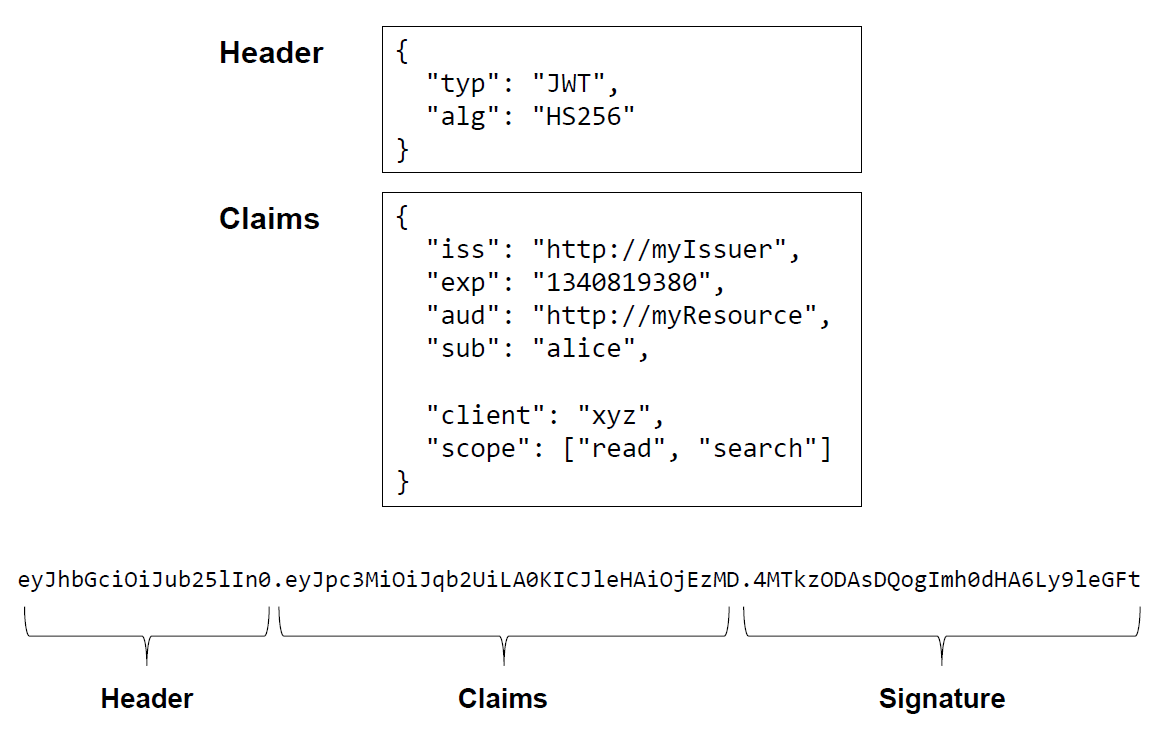
\includegraphics[width=300px]{jwt-example.png}
  \caption{Schéma expliquant la structure d'un JSON Web Token. Le jeton qui sera
    échangé entre les deux applications est la chaîne de caractère. Les parties header
    et claims résultent de l'encodage base64 des JSON respectifs. La signature
    est générée grâce à l'algorithme HS256 en utilisant une clef secrète qui
    n'est pas donnée dans ce cas.}
\end{figure}

Un exemple complet est donné sur le site officiel du standard.\cite{official-jwt-website}

La bibliothèque OCaml \emph{jwt}\cite{ocaml-jwt-github} fournit une interface
simple pour créer, chiffrer et déchiffrer un JWT.

Un token est représenté par un type abstrait \verb|t|. Le token chiffré peut
être généré grâce à la fonction \verb|token_of_t|. Le header et les différents
claims peuvent être reconstitués en JSON en utilisant la fonction
\verb|t_of_token|.

Au niveau des algorithmes de chiffrement,
\textit{Cryptokit}\cite{ocaml-cryptokit-ocaml-forge} est utilisé et uniquement
HS256 est supporté\footnote{Car uniquement cette méthode est utilisée pour OpenID
  Connect}. Les différents algorithmes sont contenus dans un type somme \verb|algorithm|.

Un header est représenté par un type abstrait \verb|header| et une valeur de ce
type peut être créé grâce à la fonction \verb|header_of_algorithm_and_type|.

Une claim est représentée par un type abstrait \verb|claim| et une liste de
claim usuel sont déjà définis (comme \emph{iss}, \emph{sub} et \emph{exp} qui
sont utilisés dans OpenID Connect). De nouveau claims peuvent être créées en
utilisant la fonction \verb|claim| qui prend le nom en paramètre. 

Le payload, c'est-à-dire l'ensemble des claims, peut être créé à travers la
valeur \verb|empty_payload| et la fonction \verb|add_claim|.
Pour obtenir les différentes claims d'un payload, la fonction \verb|find_claim|
peut être utilisée.

\subsection{Crawling de données et binding à NodeJS et NightmareJS}

\subsection{Ocsigen Start}


\subsubsection*{Push notifications}

\subsubsection*{i18n}

\subsubsection*{Tâches mineures}

\subsection{Personnelles}

A côté des heures passées dans les bureaux de Be Sport, j'ai continué à
m'intéresser au projet Ocsigen et à y contribuer. Bien que ces tâches soient
rapides, elles m'ont permis d'améliorer mes connaissances et d'être plus efficace
les jours suivants. Voici une liste non exhaustive:
\begin{itemize}
  \item eliom-distillery : option \verb|-list-templates| afin de lister tous les templates installés.
  \item eliom-distillery : option \verb|-y| pour ne pas demander de confirmation lors
    de la création d'un projet.
  \item eliom-distillery : options \verb|-add-git-template| et
\verb|-rm-template| pour permettre d'ajouter ses propres templates Eliom.\cite{eliom-distillery-repo}
  \item Binding OCaml au plugin Cordova
    \href{https://github.com/fechanique/cordova-plugin-fcm}{cordova-plugin-fcm}.\cite{ocaml-cordova-plugin-fcm} \\
    Celui-ci s'ajoute à la liste des bindings que j'ai réalisés pendant
l'année 2015-2016.\cite{ocaml-cordova-plugin-list}
\end{itemize}
